\documentclass[
	12pt,				% tamanho da fonte
	openright,			% capítulos começam em pág ímpar (insere página vazia caso preciso)
	twoside,			% twoside para impressão em verso e anverso. Oposto a oneside
	a4paper,			% tamanho do papel. 
	% -- opções do pacote babel --
	english,			% idioma adicional para hifenização
	french,				% idioma adicional para hifenização
	spanish,			% idioma adicional para hifenização
	brazil				% o último idioma é o principal do documento
	]{abntex2}

% ---
% Pacotes básicos 
% ---
\usepackage{adjustbox}
\usepackage{amsmath}
\usepackage{mathtools}
\usepackage[printonlyused]{acronym}
\usepackage{lmodern}			% Usa a fonte Latin Modern			
%\usepackage{uarial}
%\renewcommand{\familydefault}{\sfdefault}
\usepackage[T1]{fontenc}		% Selecao de codigos de fonte.
\usepackage[utf8]{inputenc}		% Codificacao do documento (conversão automática dos acentos)
\usepackage{lastpage}			% Usado pela Ficha catalográfica
\usepackage{indentfirst}		% Indenta o primeiro parágrafo de cada seção.
\usepackage{color}				% Controle das cores
\usepackage{graphicx}			% Inclusão de gráficos
\usepackage{subcaption}
\usepackage{microtype} 			% para melhorias de justificação
\usepackage[brazilian,hyperpageref]{backref}	 % Paginas com as citações na bibl
\usepackage[alf]{abntex2cite}	% Citações padrão ABNT
\usepackage[table]{xcolor}
\usepackage{multirow}
\usepackage{pgfplots} %graficos
\usepackage{booktabs,makecell}

\usepackage{array}
\newcolumntype{L}[1]{>{\raggedright\let\newline\\\arraybackslash\hspace{0pt}}m{#1}}
\newcolumntype{C}[1]{>{\centering\let\newline\\\arraybackslash\hspace{0pt}}m{#1}}
\newcolumntype{R}[1]{>{\raggedleft\let\newline\\\arraybackslash\hspace{0pt}}m{#1}}
% --- 
% CONFIGURAÇÕES DE PACOTES
% --- 

\DeclareMathOperator*{\maxi}{Maximizar}
\DeclareMathOperator*{\mini}{Minimizar }

\newcommand{\icol}[1]{% inline column vector
  \left(\begin{smallmatrix}#1\end{smallmatrix}\right)%
}

% ---
% Configurações do pacote backref
% Usado sem a opção hyperpageref de backref
\renewcommand{\backrefpagesname}{Citado na(s) página(s):~}
% Texto padrão antes do número das páginas
\renewcommand{\backref}{}
% Define os textos da citação
\renewcommand*{\backrefalt}[4]{
	\ifcase #1 %
		Nenhuma citação no texto.%
	\or
		Citado na página #2.%
	\else
		Citado #1 vezes nas páginas #2.%
	\fi}%
% ---
% ---
% Informações de dados para CAPA e FOLHA DE ROSTO
% ---
\titulo{Implementação de Algoritmos de Clusterização para Aplicação em Sequências Genômicas}
\title{Implementação de Algoritmos de Clusterização para Aplicação em Sequências Genômicas}
\autor{Álisson Rodrigues Teles}
\local{Caxias do Sul}
\data{2018}
\orientador{André Luis Martinotto}
\coorientador{}
\universidade{UNIVERSIDADE DE CAXIAS DO SUL}
\instituicao{%
UNIVERSIDADE DE CAXIAS DO SUL
\par
ÁREA DO CONHECIMENTO DE CIÊNCIAS EXATAS E ENGENHARIAS
\par
BACHARELADO EM CIÊNCIA DA COMPUTAÇÃO}

\tipotrabalho{Projeto de Diplomação}
% O preambulo deve conter o tipo do trabalho, o objetivo, 
% o nome da instituição e a área de concentração 
\preambulo{Projeto de Diplomação submetido ao curso de Bacharelado em
Ciência da Computação do Centro de Computação e Tecnologia da
Informação da Universidade de Caxias do Sul, como requisito obrigatório para graduação.}
% ---

% alterando o aspecto da cor azul
\definecolor{blue}{RGB}{41,5,195}

% informações do PDF
\makeatletter
\hypersetup{
     	%pagebackref=true,
		pdftitle={\@title}, 
		pdfauthor={\@author},
    	pdfsubject={\imprimirpreambulo},
	    pdfcreator={LaTeX with abnTeX2},
		pdfkeywords={abnt}{latex}{abntex}{abntex2}{trabalho acadêmico}, 
		colorlinks=true,       		% false: boxed links; true: colored links
    	linkcolor=blue,          	% color of internal links
    	citecolor=blue,        		% color of links to bibliography
    	filecolor=magenta,      		% color of file links
		urlcolor=blue,
		bookmarksdepth=4
}
\makeatother
% --- 

% --- 
% Espaçamentos entre linhas e parágrafos 
% --- 

% O tamanho do parágrafo é dado por:
\setlength{\parindent}{1.3cm}

% Controle do espaçamento entre um parágrafo e outro:
\setlength{\parskip}{0.2cm}  % tente também \onelineskip

% ---
% compila o indice
% ---
\makeindex
% ---

% ----
% Início do documento
% ----
\begin{document}

% Retira espaço extra obsoleto entre as frases.
\frenchspacing 

% ----------------------------------------------------------
% ELEMENTOS PRÉ-TEXTUAIS
% ----------------------------------------------------------
% \pretextual

% ---
% Capa
% ---
\imprimircapa
% ---

% ---
% Folha de rosto
% (o * indica que haverá a ficha bibliográfica)
% ---
\imprimirfolhaderosto*
% ---

% ---
% Inserir a ficha bibliografica
% ---
%% Isto é um exemplo de Ficha Catalográfica, ou ``Dados internacionais de
% catalogação-na-publicação''. Você pode utilizar este modelo como referência. 
% Porém, provavelmente a biblioteca da sua universidade lhe fornecerá um PDF
% com a ficha catalográfica definitiva após a defesa do trabalho. Quando estiver
% com o documento, salve-o como PDF no diretório do seu projeto e substitua todo
% o conteúdo de implementação deste arquivo pelo comando abaixo:
%
% \begin{fichacatalografica}
%     \includepdf{fig_ficha_catalografica.pdf}
% \end{fichacatalografica}
\begin{fichacatalografica}
	\vspace*{\fill}					% Posição vertical
	\hrule							% Linha horizontal
	\begin{center}					% Minipage Centralizado
	\begin{minipage}[c]{12.5cm}		% Largura
	
	\imprimirautor
	
	\hspace{0.5cm} \imprimirtitulo  / \imprimirautor. --
	\imprimirlocal, \imprimirdata-
	
	\hspace{0.5cm} \pageref{LastPage} p. : il. (algumas color.), 30 cm.\\
	
	\hspace{0.5cm} \imprimirorientadorRotulo~\imprimirorientador\\
	
	\hspace{0.5cm}
	\parbox[t]{\textwidth}{\imprimirtipotrabalho~--~\imprimirinstituicao,
	\imprimirdata.}\\
	
	\hspace{0.5cm}
		1. AMQP.
		2. \textit{Analytic Hierarchy Process}.
		I. André Luis Martinotto.
		II. Universidade de Caxias do Sul.
		III. Faculdade de Ciências da Computação.
		IV. Avaliação de intermediadores de mensagem que implementam o protocolo \textit{AMQP}\\ 			
	
	\hspace{8.75cm} CDU 02:141:005.7\\
	
	\end{minipage}
	\end{center}
	\hrule
\end{fichacatalografica}
% ---

% ---
% Inserir folha de aprovação
% ---
%% Isto é um exemplo de Folha de aprovação, elemento obrigatório da NBR
% 14724/2011 (seção 4.2.1.3). Você pode utilizar este modelo até a aprovação
% do trabalho. Após isso, substitua todo o conteúdo deste arquivo por uma
% imagem da página assinada pela banca com o comando abaixo:
%
% \includepdf{folhadeaprovacao_final.pdf}
%
\begin{folhadeaprovacao}

  \begin{center}
    {\ABNTEXchapterfont\large\imprimirautor}

    \vspace*{\fill}\vspace*{\fill}
    \begin{center}
      \ABNTEXchapterfont\bfseries\Large\imprimirtitulo
    \end{center}
    \vspace*{\fill}
    
    \hspace{.45\textwidth}
    \begin{minipage}{.5\textwidth}
        \imprimirpreambulo
    \end{minipage}%
    \vspace*{\fill}
   \end{center}
        
   Trabalho aprovado. \imprimirlocal, 13 de dezembro de 2018: 

   \assinatura{\textbf{\imprimirorientador} \\ Orientador} 
   \assinatura{\textbf{Daniel Luís Notari} \\ Convidado 1}
   \assinatura{\textbf{Helena Graziottin Ribeiro} \\ Convidado 2}
   \begin{center}
    \vspace*{0.5cm}
    {\large\imprimirlocal}
    \par
    {\large\imprimirdata}
    \vspace*{1cm}
  \end{center}
  
\end{folhadeaprovacao}
% ---

% ---
% Dedicatória
% ---
%\include{diversos/dedicatoria}
% ---

% ---
% Agradecimentos
% ---
%\include{diversos/agradecimentos}
% ---

% ---
% RESUMOS
% ---
%% resumo em português
\setlength{\absparsep}{18pt} % ajusta o espaçamento dos parágrafos do resumo
\begin{resumo}

As redes sociais estão cada vez mais inseridas no cotidiano das pessoas. Essas ferramentas trazem melhoria na comunicação e disseminação de opiniões, permitindo que várias culturas se unam em meio a postagens sobre os mais variados assuntos. Os brasileiros estão cada vez mais inseridos nos meios tecnológicos e são ativos usuários dessas redes sociais. Contudo, com a liberdade de expressão vieram comportamentos agressivos de preconceito, os discursos de ódio, tendo como alvos mulheres, deficientes, negros e muçulmanos, espalhando ódio e assédios verbais. O controle sobre postagens violentas e de assédio moral é normalmente realizado de forma manual. O uso de ferramentas automatizadas pode auxiliar e facilitar esta tarefa. Com base nisso, o trabalho pretende abordar a Análise de Sentimentos aplicada às redes sociais para detectar discursos de ódio de raça, gênero, religião, e deficiência, especificamente na língua portuguesa. Este tema é relevante já que poucos trabalhos têm abordado a Análise de Sentimentos e geração de base de léxicos para o idioma português. Ao longo deste trabalho pretende-se gerar um dicionário léxico, contendo termos da língua portuguesa, para uso na detecção de \textit{haters}. Tal léxico será usado em um software específico, que uma vez integrado ao \textit{Twitter}, será testado e avaliado.
%Os resultados obtidos serão comparados com uma aplicação de Redes Neurais Artificiais empregada com o mesmo propósito de classificação.

 \textbf{Palavras-chaves}: Análise de Sentimentos, Discurso de Ódio, Twitter, Haters, Weka
\end{resumo}

% resumo em inglês
\begin{resumo}[Abstract]
 \begin{otherlanguage*}{english}
   Social networks are increasingly inserted in people's daily lives. These tools bring improvement in communication and dissemination of opinions, allowing multiple cultures to come together amid postings on the most varied subjects. Brazilians are increasingly inserted in the technological media and are active users of these social networks. However, with freedom of expression came aggressive behavior of prejudice, hate speech, targeting women, disabled, blacks and Muslims, spreading hatred and verbal harassment. Control over violent posting and bullying is usually done manually. The use of automated tools can help and facilitate this task. Based on this, the work intends to approach the sentiment analysis applied to social networks to detect hate speech of race, gender, religion, and disability, specifically in the Portuguese language. This topic is relevant since few studies have dealt with the sentiment analysis and generation of a base of lexicons for the Portuguese language. Throughout this work we intend to generate a lexical dictionary, containing terms of the Portuguese language, for use in the detection of haters. This lexicon will be used in a specific software, which once integrated with Twitter, will be tested and evaluated.

   \vspace{\onelineskip}
 
   \noindent 
   \textbf{Keywords}: Sentiment Analysis, Hate Speech, Twitter, Haters, Weka
 \end{otherlanguage*}
\end{resumo}

% ---

% ---
% inserir lista de ilustrações
% ---
\pdfbookmark[0]{\listfigurename}{lof}
\listoffigures*
\cleardoublepage
% ---

% ---
% inserir lista de tabelas
% ---
\pdfbookmark[0]{\listtablename}{lot}
\listoftables*
\cleardoublepage
% ---

% ---
% inserir lista de abreviaturas e siglas
% ---
\begin{siglas}
   \item[ATE]{\textit{Automatic Term Expansion}}
   \item[CURE]{\textit{Clustering Using Representatives}}
   \item[DNA]{\textit{Deoxyribonucleic acid}}
   \item[DWT]{\textit{Discrete Wavelet Transform}}
   \item[EM]{\textit{Expectation-Maximization Clustering}}
   \item[HGKA]{\textit{Hibrid Genetic k-means Algorithm}}
   \item[MUSA]{\textit{Motif Finding Using na Unsupervised Approach}}
   \item[TCC]{\textit{Trabalho de Conclusão de Curso}}
\end{siglas}
% ---
% inserir o sumario
% ---
\pdfbookmark[0]{\contentsname}{toc}
\tableofcontents*
\cleardoublepage
% ---

% ----------------------------------------------------------
% ELEMENTOS TEXTUAIS
% ----------------------------------------------------------
\textual

%\chapter{Introdução}
\label{cap:Introducao}
% contextualizar 
Com a globalização do uso da \textit{internet}, a sociedade aprimorou a sua forma de interagir e desenvolveu novas ferramentas para as relações interpessoais, profissionais e etc. Essas ferramentas são chamadas de redes sociais e são exemplos o \textit{Facebook}\footnote{\url{https://www.facebook.com}}, o \textit{Twitter}\footnote{\url{https://twitter.com}} e o \textit{Instagram}\footnote{\url{https://www.instagram.com}} entre outros no mercado. Essas ferramentas estão presentes na maioria dos \textit{smartphones} da população, e a cada dia aumentam o número de usuários ativos em suas plataformas. Segundo pesquisa realizada pelo \citeonline{ibge2018}, $64,7\%$ das pessoas de 10 anos ou mais utilizaram a \textit{internet} e $94,6\%$ das conexões foram realizadas por \textit{smartphones}. Ainda na mesma pesquisa foi verificado que $94,2\%$ da finalidade dessas conexões foi enviar ou receber mensagens de texto, áudio ou imagens por aplicativos diferentes de \textit{e-mail}. Dentro dessas inúmeras publicações existem muitos conteúdos que são de interesse comum da população já que a mesma está compartilhando seu conhecimento, crítica e opinião aumentando a participação nos mais variados assuntos, desde opinião sobre determinado produto até descontentamento social, há também riscos de agressão verbal entre os membros das comunidades e, o gerenciamento manual acaba sendo impossível devido ao número de dados gerados a cada dia.

% falar sobre o desafio na área 
Para realizar a análise textual dessa imensa quantidade de dados é necessário o uso de recursos computacionais já que a análise manual se torna impraticável  pela demora no tempo de resposta. O número crescente de opiniões também gerou o interesse de grandes empresas em garimpar grupos públicos em interpretar os sentimentos manifestados de seus usuários para verificar aprovação de seus produtos sem necessitar de pesquisas pessoais e até invasivas, diminuindo gastos e acelerando as conclusões para tomadas de decisões. Além disso, há uma necessidade de ferramentas que realizem a análise tendo como base a língua portuguesa já que existem poucas com resultados satisfatórios e poucas pesquisas relacionadas ao idioma.

% apresentar solução
É Nesse contexto que se desenvolve a técnica de \textit{Sentiment Analysis}, uma subárea da TDM (\textit{Text Data Mining})\cite{Hearst:1999:UTD:1034678.1034679}, que se refere ao processo de extrair padrões (conhecimentos de interesse das mais variadas áreas de pesquisa) de documentos textuais não estruturados tendo enfase na detecção das emoções envolvidas nessas produções que podem ter seus sentimentos classificados em: positivos, negativos e neutros. \cite{Li:2010:SAG:2898607.2898826}. 

%bebefícios na area 
As vantagens em fazer pesquisa de opinião por meio de \textit{Sentiment Analysis} são: o baixo custo de análise, rapidez de pesquisa e resposta, autenticidade e não invasão. Sendo os últimos dois itens os maiores diferenciais da técnica pelo fato de as informações usadas como objeto de estudo serem buscadas de comunidades públicas e de a veracidade das informações ser natural já que os usuários não são previamente avisados sobre a pesquisa a ser realizada. Trazendo avanços para a indústria, órgãos públicos, e até mesmo para o indivíduo essa é uma área de pesquisa em crescimento sendo também crescente o interesse em ferramentas ágeis para resultados em tempo real. 

A mesma liberdade de expressão que a \textit{internet} proporcionou deu lugar para que pessoas também utilizem as redes sociais para propagar discursos de ódio contra grupos de minoria. Tornando a \textit{internet} também um lugar hostil com agressões verbais \cite{Chetty2018}.  Além disso, poucos trabalhos abordaram o tema contextualizando o problema na língua portuguesa tornando esse um tema distante e silencioso.

\section{Objetivos}
\subsection{Objetivo Geral}    
    Esse trabalho tem por objetivo desenvolver e avaliar um \textit{software} de detecção de \textit{haters} baseado em Análise de Sentimentos expressos em textos na Língua Portuguesa. 

\subsection{Objetivos Específicos}
    Para atingir o objetivo geral serão seguidos os seguintes objetivos específicos:
\begin{enumerate}
    \item Identificar métodos computacionais para a Análise de Sentimentos e detecção de \textit{haters}.
    \item Implementar um método para detecção de \textit{haters} em dados textuais.
    \item Realizar testes do \textit{software} desenvolvido, comparando os resultados com análises feitas por especialistas humanos.
    \item Avaliar o desempenho do método implementado.
\end{enumerate}
	
\section{Organização do Documento}
O restante do trabalho é organizado da seguinte maneira:

\begin{itemize}

\item \textbf{Capítulo \ref{cap:REFERENCIAL} - Revisão Bibliográfica:} Compreende toda a fundamentação teórica necessária para o desenvolvimento e entendimento do estudo apresentado. É apresentado as etapas principais desenvolvidas em uma análise de sentimento, bem como os principais algoritmos utilizados na classificação dos textos, uma breve explicação dos conceitos de redes sociais, além de estudo de discurso de ódio dentro dessas plataformas. Alguns trabalhos relacionados também são citados no final do capítulo.

\item \textbf{Capítulo \ref{cap:Desenvolvimento} - Desenvolvimento:} São apresentadas as etapas previstas, bem como a metodologia utilizada no desenvolvimento do trabalho tendo o objetivo de criar uma base de léxicos contidos em discursos de ódio, a integração com \textit{software} já desenvolvido que realiza Análise de Sentimentos baseado em emoções e a verificação da efetividade nas detecções de discursos de ódio.

\item \textbf{Capítulo \ref{cap:conclusoes} - Conclusões:} É apresentada síntese do trabalho desenvolvido até então, bem como projeção de atividade futuras em cronograma de atividades detalhado no final do capítulo.
\end{itemize}

\chapter{Problema}
\label{cap:PROBLEMA}

A Biologia vem sendo uma ciência observacional e não dedutiva e mesmo que atualmente essa orientação básica não tenha sido alterada, a natureza dos dados mudou radicalmente. Com o progresso das pesquisas biológicas os dados de fato cresceram em quantidade e em precisão.\cite{lesk2005introduction}.


\section{Problema de Pesquisa}
% conceituar usuário sobre o problema de pesquisa
% Para contribuir com o avanço no estudo e manipulação dos dados biológicos, ciências como Matemática, a própria Biologia, Ciência da Computação e outras demais ciências unificaram-se dando origem a Biotecnologia sendo que, para  as funções computacionais, foi criada a Bioinformática. 
%aqui posso tratar dos bancos de dados e suas propriedades e depois falar do problema da demora de consulta de padrões 

Atualmente há uma grande movimentação científica no que diz respeito ao mapeamento genético dos seres vivos e grandes bancos de dados, sejam públicos ou privados, são mantidos por pesquisadores participantes da comunidade acadêmica e também pesquisadores autônomos. O estudo das funções gênicas é uma das principais linhas de pesquisa da Biologia e da Bioinformática pois com o amadurecimento das mesmas será possível compreender os processos moleculares e bioquímicos que melhoram nossa saúde e que causam doenças, para a fabricação de novos remédios e diagnósticos mais confiáveis\cite{Murali2006}. 

Para manipular essas informações e buscar padrões de similaridade genômica, muitas ferramentas computacionais vem sendo desenvolvidas. Elas usam  a combinação de procedimentos matemáticos, estatísticos e de programação. Tudo isso para garantir assertividade já que a sequencia de \textit{DNA} é uma estrutura complexa e crescente.

%posso citar as pesquisas da ucs e depois questionar 

\section{Questão de Pesquisa}
% realizar pergunta a ser respondida com o TCC
Baseado no problema de pesquisa abordado na sessão anterior, foi criada a seguinte questão de pesquisa: É possível acelerar a busca por regiões promotoras e terminadoras de uma mesma base de dados públicos de \textit{DNA} usando técnicas robustas de \textit{clustering}? Os progressos computacionais com a implementação dos novos métodos tornará a ferramenta já implementada pela Universidade de Caxias do Sul mais performática quando exigido um maior número de \textit{clusters}\cite{Basso:2015:UCS}\cite{Fontana:2013:UCS}? 
%falar aqui depois sobre a distribuição dos capítulos
% ----------------------------------------------------------
% REFERENCIAIS TEORICOS
% ----------------------------------------------------------
\part{Referenciais teóricos}
\chapter{Programa de Clusterização de Análise Genômica}
\label{cap:PROGRAMA}

Tendo em vista o progresso nos estudos de Bioinformática e a busca por melhoria, mais especificamente, nas análises genômicas de \textit{DNA}, em sua tese, Eduardo Andreetta Fontana desenvolveu uma ferramenta que aplica os conceitos de clusterização na análise genômica da bactéria \textit{Escherichia Coli} (\textit{E. coli}) diferenciando regiões promotoras, terminadoras e do gene propriamente dito. Na mesma, o autor desenvolve os algoritmos \textit{K-Means} e \textit{CURE} (\textit{Clustering Using Representatives}) e usa como base de dados o banco de dados público \textit{RegulonDB}\cite{Fontana:2013:UCS}.

No final de seus estudos, Fontana concluiu que teve resultados relevantes para vetores de 2\(\mathit{n}\) e 3\(\mathit{n}\) sendo que sua proposta era clusterizar todos os segmentos em vetores de 2\(\mathit{n}\) até 10\(\mathit{n}\) mas nesses últimos casos a ferramenta mostrou tempo de execução além da viabilidade aceitável. Tal resultado foi atribuído a natureza complexa e ruidosa da representação dos dados biológicos\cite{Fontana:2013:UCS}.

O autor visionou a necessidade de enfoque na exploração da fase de extração de atributos já que a mesma é determinante para a definição dos atributos característicos de qualquer objeto de estudo, Fontana sugeriu estudos utilizando a teoria de \textit{ATE} (\textit{Automatic Term Expansion}) \cite{Ji:2008} para a contabilização de frequência de termos, além disso sugeriu outros complementos como gráficos de dendrograma para representações \textit{CURE}, erro quadrático para \textit{K-Means} e alinhamentos de sequência para cada \textit{cluster}\cite{Fontana:2013:UCS}.

Dois anos mais tarde Thiago Angelo Basso realizou em sua tese o estudo focado na fase de seleção e extração de atributos suavizando os ruídos até então constatados e implementando os mesmos na ferramenta desenvolvida por Fontana, significando um complemento no estudo das expressões genicas com algoritmos de clusterização. \cite{Basso:2015:UCS}.

Foi constatado que a abordagem \textit{ATE} elevou os pesos dos atributos com maior grau de correlação entre as sequências mas que não influenciou na etapa de clusterização, com a abordagem \textit{MUSA}\cite{Mendes2006} constatou que a mesma é eficiente na identificação de motivos mas por gerar um esforço computacional grande não é uma boa escolha para a seleção de centroides iniciais. já na fase de extração o autor propôs uma solução em séries temporais utilizando \textit{DWT}\cite{Batal2009} e verificou que a abordagem foi satisfatória já que foi possível suavizar as series temporais e assim melhorar consideravelmente o agrupamento dos \textit{clusters} na fase de clusterização\cite{Basso:2015:UCS}.

Com a ideia de progredir os estudos da análise genômica Basso propôs otimizações no algoritmo \textit{MUSA}, técnicas de extração de atributos também foram sugeridas, como por exemplo o algoritmo \textit{HGKA} afim de eliminar a dependência de inicialização\cite{Basso:2015:UCS}.

Hoje a ferramenta é amplamente usada pela comunidade acadêmica da Universidade de Caxias do Sul e, graças as pesquisas descritas anteriormente, os alunos de graduação em Biologia que atuam como bolsistas de iniciação científica realizam as pesquisas de expressões genômicas de uma forma mais ágil que as abordagens tradicionais.
 
%verificar referencias para HGKA
%apresentar tabelas de resultados de cada um deles?





















\chapter{Clusterização}
\label{cap:CLUSTERIZACAO}

Clusterização, ou ainda, análise de Cluster é a classificação não-supervisionada de padrões (sejam eles dados recolhidos, observações, ou ainda, vetores de atributos) em grupos concentrados chamados de \textit{Cluster}. Um exemplo de clusterização é apresentado na Figura \ref{fig:DATA-CLUSTERING}\cite{Jain:1999:DCR:331499.331504}, onde na Figura \ref{fig:DATA-CLUSTERING}(a) é apresentado o cojunto de informações de entrada e na Figura \ref{fig:DATA-CLUSTERING}(b) é apresentado o resultado de agrupamento dos dados analisados.

\begin{figure}[!h]
\centering 
\caption{Exemplo de Clusterização}
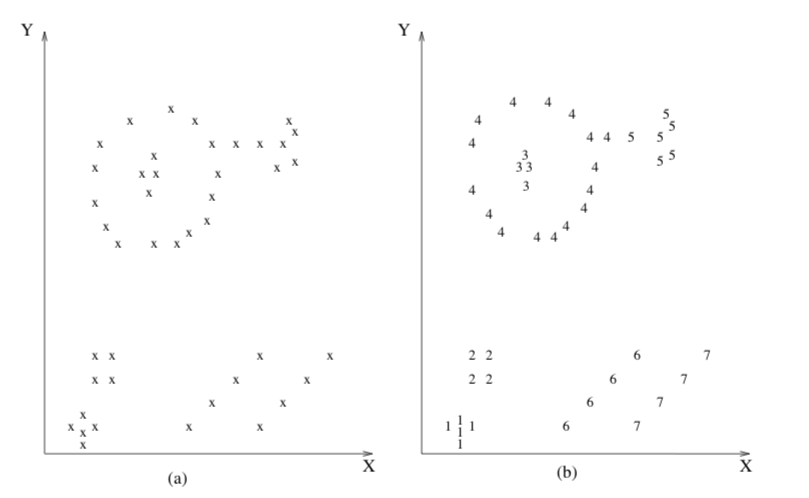
\includegraphics[width = \textwidth]{imagens/dataclustering.png}
\legend{Fonte: \citeauthor{Jain:1999:DCR:331499.331504}}
\label{fig:DATA-CLUSTERING}
\end{figure}

%A diferença entre clusterização (classificação não-supervisionada) e análise descriminante (classificação supervisionada) é que na segunda classificação os padrões estão rotulados 

Hoje a clusterização representa uma das principais etapas de análise de dados e é amplamente abordada em muitos contextos e por vários pesquisadores em suas disciplinas. Por conta do uso multidisciplinar e também a contextualização em diferentes comunidades, as metodologias, termos e até fases de implementação recebem nomes distintos da área de aplicação dos seus algoritmos.

A Clusterização é muito usada em análises exploratórias de padrão, agrupamento de dados, tomadas de decisão e muitas situações de \textit{Machine Learning} incluindo \textit{Data Mining}, recuperação de documentos, segmentação de imagens e classificação de padrões.

\section{Componentes de uma Tarefa de Clusterização}

A Clusterização tem esses passos como principais para o agrupamentos de objetos:
\begin{enumerate}
\item \textit{representação de padrões}: Fase em que se inclui, opcionalmente, a extração de atributos e ou extração de seleção. Aqui ocorre a a análise da classe, tipo, número e escala dos atributos que são importantes para o processo de clusterização. A seleção de atributos é a busca dos atributos mais efetivos e a extração de atributos é quando se faz necessário uma ou mais transformações dos atributos originais para gerar atributos mais notáveis para o \textit{clustering};

\item \textit{definição de uma medida de proximidade de padrões (sendo essa medida adequada aos dados observados)}: Fase que geralmente mede a distância entre pares de padrões. Para o cálculo simples entre dois atributos pode ser utilizada a distância Euclidiana. Já para outros cálculos de distância, outras fórmulas de distância são necessárias;

\item \textit{clusterização ou agrupamento}: Fase que pode ser desempenhada de varias formas. O agrupamento pode ser classificado como \textit{crisp} (onde cada padrão pertence ou não a um determinado grupo) ou \textit{fuzzy} (onde cada padrão pode apresentar graus de relacionamento com os grupos). Os algoritmos de clusterização hierárquica produz séries de partições aninhadas onde os objetos se unem ou se separam levando como critério a similaridade de seus atributos. Os algoritmos de clusterização particional identificam as melhores partições sendo otimizadas a cada iteração com base nos critérios de agrupamento.; 

\item \textit{apresentação dos resultados}: Fase que extrai os resultados da clusterização para uma linguagem simplificada e de fácil interpretação quando é um processo humano-orientado ou com atributos úteis e de melhor processamento quando é um processo automatizado;
\end{enumerate}

\begin{figure}[!h]
\centering 
\caption{Tarefas de Clusterização}
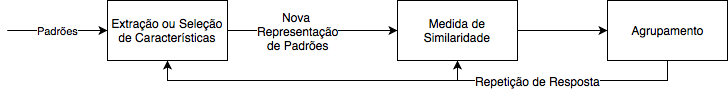
\includegraphics[width = \textwidth]{imagens/fasesclusterizacao.png}
\legend{Fonte: \citeauthor{Jain:1999:DCR:331499.331504}}
\label{fig:FASES-CLUSTERIZACAO}
\end{figure}

\newpage

\section{Definições e Notação}
Essa sessão tem o objetivo de apresentar as definições básicas e as notações que serão utilizadas nas sessões seguintes.

\begin{enumerate}
\item Padrão (ou ainda, vetor de atributos) \textbf{x} é um item único usado pelo algoritmo de clusterização. Geralmente é um vetor de $\mathit{d}$ medidas: $\mathbf{x}= (x_{1}, ..., x_{d})$.

\item O componente escalar $x_{i}$ do padrão \textbf{x} é chamado de característica ou atributo.

\item $\mathit{d}$ é chamado de dimensionalidade do padrão ou do espaço do padrão.

\item O conjunto padrão é denotado por $X= \left\{ \mathbf{x}_{1}, ...,\mathbf{x}_{n}\right\}$. O padrão $i$ em $X$ é denotado por $\mathbf{x_i}= (x_{i,1}, ..., x_{i,d})$. Há casos em que o conjunto padrão é uma matriz de padrões com as dimensões $n\times d$.

\item Classe é um estado que reflete características de um objeto e ou de um grupo com similaridades. Cada classe apresentada após o uso de uma técnica de clusterização reflete um grupo contido no conjunto padrão inicial da análise.

\item A técnica \textit{crisp} assume um rótulo de classe $l$ para cada padrão $\mathbf{x_i}$. O conjunto para todos os rótulos para um conjunto padrão $X$ é $L=\left\{l_1, ..., l_n\right\}$ com $l_i \in \left\{1, ..., k\right\}$, onde $k$ é o número de \textit{clusters}.

\item A técnica \textit{fuzzy} assume para cada padrão $\mathbf{x_i}$ uma fração $f_i,j$ que expressa o grau de associação em cada \textit{cluster} $j$.  
\end{enumerate}

%\include{capitulos/3-deteccao-doencas}
%\include{capitulos/4-svm}

% ----------------------------------------------------------
% RESULTADOS
% ----------------------------------------------------------
%\part{Proposta de solução}
%\include{capitulos/5-proposta}
%\include{capitulos/5-implementacao}
%\include{capitulos/6-consideracoes}

% ----------------------------------------------------------
% RESULTADOS
% ----------------------------------------------------------
%\part{Resultados}

%\include{capitulos/capitulo1}

% ----------------------------------------------------------
% Finaliza a parte no bookmark do PDF
% para que se inicie o bookmark na raiz
% e adiciona espaço de parte no Sumário
% ----------------------------------------------------------
%\phantompart

% ---
% Conclusão (outro exemplo de capítulo sem numeração e presente no sumário)
% ---
%\chapter*[Conclusão]{Conclusão}
%\addcontentsline{toc}{chapter}{Conclusão}
% ---


% ----------------------------------------------------------
% ELEMENTOS PÓS-TEXTUAIS
% ----------------------------------------------------------
\postextual
% ----------------------------------------------------------

% ----------------------------------------------------------
% Referências bibliográficas
% ----------------------------------------------------------
\bibliographystyle{abntex2-alf}
\bibliography{tcc}

% ----------------------------------------------------------
% Glossário
% ----------------------------------------------------------
%
% Consulte o manual da classe abntex2 para orientações sobre o glossário.
%
%\glossary

% ----------------------------------------------------------
% Apêndices
% ----------------------------------------------------------

% ---
% Inicia os apêndices
% ---
%\include{diversos/apendices}
% ---


% ----------------------------------------------------------
% Anexos
% ----------------------------------------------------------
%\include{diversos/anexos}

%---------------------------------------------------------------------
% INDICE REMISSIVO
%---------------------------------------------------------------------
%\phantompart
%\printindex
%---------------------------------------------------------------------

\end{document}
